\documentclass[12pt,twoside]{report}

\usepackage[utf8]{inputenc}
\usepackage[spanish]{babel}

\usepackage{amsmath}
\usepackage{amsfonts}
\usepackage{amssymb}

\usepackage{setspace}

\usepackage{enumitem}

\usepackage[normalem]{ulem}

\usepackage[table,xcdraw]{xcolor}

\usepackage[export]{adjustbox}
\usepackage[official]{eurosym}
\usepackage{longtable}

\usepackage{wrapfig}

%%%%%%%%%%%%%%%%%%%%%%%%%%%%%%%%%%%%%%%%%%%%%%%%%%%%%%%%%%%%%%%%%%%%%%%%%%%%%

% Definitions for the title page
\newcommand{\reporttitle}{
	Propuesta de Actividades \\y Solicitud de Subvención
}
\newcommand{\reportauthor}{Asociación Club de Robótica-Mecatrónica}



\setlength{\parskip}{\baselineskip}
\setlength{\parindent}{0pt}

\usepackage{hyperref}
\hypersetup{
    linktoc=page, breaklinks,
    pdfauthor=\reportauthor,pdftitle={Memoria de Actividades}
}
%%%%%%%%%%%%%%%%%%%%%%%%%%%%%%%%%%%%%%%%%%%%%%%%%%%%%%%%%%%%%%%%%%%%%%%%%%%%%

% load some definitions and default packages
%%%%%%%%%%%%%%%%%%%%%%%%%%%%%%%%%%%%%%%%%
% University Assignment Title Page 
% LaTeX Template
% Version 1.0 (27/12/12)
%
% This template has been downloaded from:
% http://www.LaTeXTemplates.com
%
% Original author:
% WikiBooks (http://en.wikibooks.org/wiki/LaTeX/Title_Creation)
%
% License:
% CC BY-NC-SA 3.0 (http://creativecommons.org/licenses/by-nc-sa/3.0/)
% 
%
%%%%%%%%%%%%%%%%%%%%%%%%%%%%%%%%%%%%%%%%%
%----------------------------------------------------------------------------------------
%	PACKAGES AND OTHER DOCUMENT CONFIGURATIONS
%----------------------------------------------------------------------------------------
%\usepackage[a4paper,left=2.8cm,right=2.8cm,vmargin=2.0cm,includeheadfoot]{geometry}
\usepackage[a4paper,left=3.5cm,right=2.1cm,vmargin=2.0cm,includeheadfoot]{geometry}

\usepackage{textpos}

\usepackage{tabularx,longtable,multirow,subfigure,caption}
\usepackage{fncylab} %formatting of labels
\usepackage{fancyhdr} % page layout
\usepackage{url} % URLs

\usepackage{amsmath}
\usepackage{graphicx}
\usepackage{dsfont}

\usepackage{array}
\usepackage{latexsym}



%%% Default fonts
\renewcommand*{\rmdefault}{bch}
\renewcommand*{\ttdefault}{cmtt}



%%% Default settings (page layout)
\setlength{\parindent}{0em}  % indentation of paragraph

\setlength{\headheight}{14.5pt}
\pagestyle{fancy}
\renewcommand{\chaptermark}[1]{\markboth{\chaptername\ \thechapter.\ #1}{}} 

\fancyfoot[EL,OR]{\sffamily\textbf{\thepage}}%Page no. in the left on odd pages and on right on even pages
\fancyfoot[OC,EC]{\sffamily }
\renewcommand{\headrulewidth}{0.1pt}
\renewcommand{\footrulewidth}{0.1pt}
\captionsetup{margin=10pt,font=small,labelfont=bf}


%--- chapter heading

\def\@makechapterhead#1{%
  \vspace*{10\p@}%
  {\parindent \z@ \raggedright \sffamily
    \interlinepenalty\@M
    \Huge\bfseries \thechapter \space\space #1\par\nobreak
    \vskip 30\p@
  }}

%---chapter heading for \chapter*  
\def\@makeschapterhead#1{%
  \vspace*{10\p@}%
  {\parindent \z@ \raggedright
    \sffamily
    \interlinepenalty\@M
    \Huge \bfseries  #1\par\nobreak
    \vskip 30\p@
  }}

\allowdisplaybreaks


\date{Marzo de 2016}

\addto\captionsspanish{\renewcommand{\chaptername}{Parte}}

\begin{document}

\begin{titlepage}

\newcommand{\HRule}{\rule{\linewidth}{1mm}} % Defines a new command for the horizontal lines, change thickness here


%----------------------------------------------------------------------------------------
%	LOGO SECTION
%----------------------------------------------------------------------------------------


\includegraphics[width = 6cm]{fotos/logo-eps.png}
\hfill

\includegraphics[width = 6cm]{fotos/logo-uam.png}



\center % Center remainder of the page

%----------------------------------------------------------------------------------------
%	HEADING SECTIONS
%----------------------------------------------------------------------------------------

%\textsc{\Large Escuela Politécnica Superior}\\[0.1cm]
%\textsc{\Large Universidad Autónoma de Madrid}\\[0.5cm]
\vspace{1cm}

%----------------------------------------------------------------------------------------
%	TITLE SECTION
%----------------------------------------------------------------------------------------


\HRule \\[0.4cm]
\begin{spacing}{1.5}
{ \fontsize{0.8cm}{1em} \bfseries \reporttitle}\\ % Title of your document
\vspace{0.5cm}
{ \fontsize{0.7cm}{1em} \bfseries \reportauthor} \\
\end{spacing}
\HRule \\[1.5cm]



\includegraphics[width = 7cm]{fotos/logo_crm-192x192.png}

{\large Asociación Club de Robótica-Mecatrónica (CRM-UAM)} \\
Local B-111 -- Escuela Politécnica Superior

\vfill

\textsc{\Large Universidad Autónoma de Madrid}\\[0.5cm]

\vfill

%----------------------------------------------------------------------------------------
%	FOOTER & DATE SECTION
%----------------------------------------------------------------------------------------


\makeatletter
{ \Large \@date }
\vfill
\makeatother


\end{titlepage}

\clearpage{\pagestyle{empty}\cleardoublepage}


% page numbering etc.
\pagenumbering{roman}
\setcounter{page}{1}
\pagestyle{fancy}






\begin{spacing}{0.1}
\tableofcontents
\end{spacing}

\clearpage{\pagestyle{empty}\cleardoublepage}

\pagenumbering{arabic}
\setcounter{page}{1}

\fancyhead[LE,RO]{\slshape}
%\fancyhead[LE,RO]{\slshape \rightmark}
\fancyhead[LO,RE]{\slshape \leftmark}

%%%%%%%%%%%%%%%%%%%%%%%%%%%%%%%%%%%%



\chapter{Propuesta de actividades}

Desde Enero ya hemos organizado 3 ``Viernes Abiertos'' y una Mini-Arduparty, con los que poco a poco estamos consiguiendo mayor visibilidad entre los estudiantes. Hay mas información en nuestro blog: \url{http://crm.ii.uam.es/blog}

\begin{wrapfigure}{R}{0.45\textwidth}
\centering
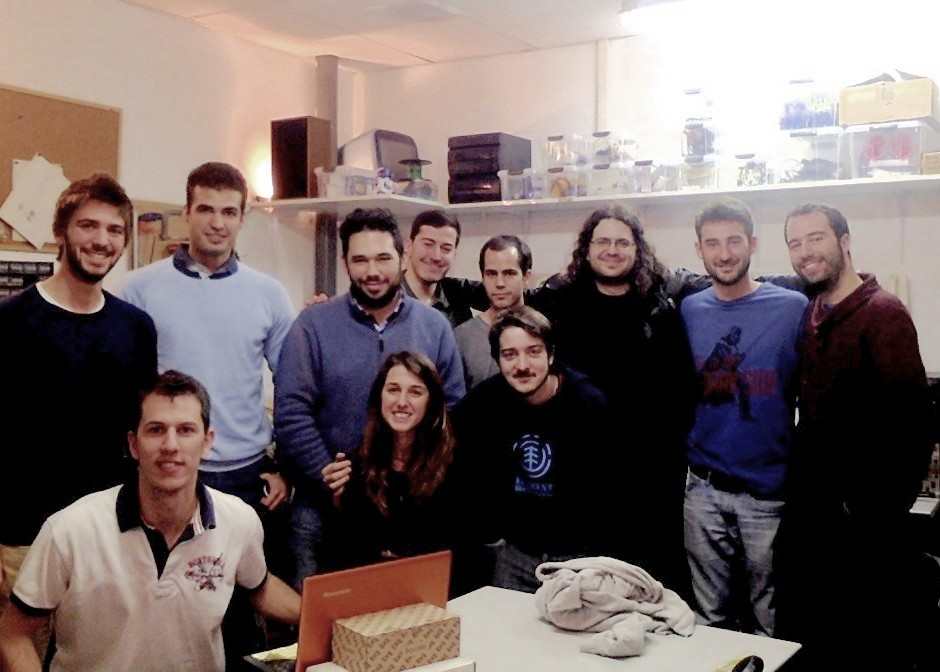
\includegraphics[width=0.44\textwidth]{fotosNuevas/acta9feb2016_b}
\caption*{Reunión de la junta del 9/Feb/2016}
\end{wrapfigure}

Recientemente instalamos en nuestro local B-111 de la EPS, gracias al nuevo material, un sistema domótico con enchufes inalámbricos que detecta cuando se accede a nuestro local, y activa automáticamente todos los enchufes y luces adicionales. Esta renovación fomenta la seguridad y el ahorro energético, ya que se desactivan automáticamente los radiadores y las estaciones de soldadura cuando no se está utilizando el local.
También hemos conseguido que el CAU nos instale por fin una antena Eduroam, lo que ha mejorado notablemente la cobertura WiFi. Esto, sumado al equipo de música que hemos reparado, resulta en un entorno de trabajo muy cómodo y productivo, que empieza a ser utilizado regularmente por los estudiantes para realizar sus proyectos.

Los proyectos que estamos desarrollando actualmente son el del coche RC autónomo\footnote{\url{https://github.com/CRM-UAM/coche-RC}}, 
mejoras del cuadrucóptero\footnote{\url{https://github.com/CRM-UAM/cuadricoptero}}, así como robots para resolver laberintos\footnote{\url{https://github.com/CRM-UAM/CRMaze}} y seguidores de línea de competición\footnote{\url{https://github.com/CRM-UAM/Vector9000}} con los que esperamos participar en la Liga Nacional de Robótica (estamos atentos para participar en los próximos eventos).


\section{Proyectos varios}

\subsection{Presupuesto para mas cajas de proyecto para los miembros}

Aunque ya hemos comprado varias cajas para la renovación del local con el presupuesto que se nos concedió con anterioridad, ya las hemos llenado todas y necesitamos algunas mas de cara al resto de proyectos van a ir surgiendo durante el año:

\begin{itemize}
\item \textbf{Cajas organizadoras transparentes grandes (21x30x40cm)}, que cuestan 4.25\euro{}/u. Estimamos necesarias 5 cajas, lo que hace un total de 21.25\euro{}
\item \textbf{Cajas de proyecto pequeñas (14x19x29cm)}, que cuestan 2.95\euro{}/u. Estimamos necesarias 20 cajas, lo que hace un total de 59\euro{}
\end{itemize}

Por tanto, para dicha compra estimamos necesarios \textbf{80.25\euro{}}.




\subsection{Construcción de un avión RC autónomo de bajo coste}

\subsubsection{Equipo de trabajo}
\begin{itemize}
\item Carlos García, estudiante de doctorado, EPS.
\item Rodrigo Jiménez, estudiante de Telecomuniciones, EPS.
\item Jaime Aragón, estudiante de Telecomuniciones, EPS.
\end{itemize}
\subsubsection{Descripción}
Hemos localizado un diseño de avión radio-control muy interesante debido a su bajo coste. Su construcción es sencilla: es posible recortar una lámina de plástico corrugado usando los planos disponibles en internet\footnote{\url{http://mugi.co.uk/evo_plans.php}}, para obtener un perfil de ala "delta" muy eficiente en vuelo.

\begin{figure}[hbtp]
\centerline{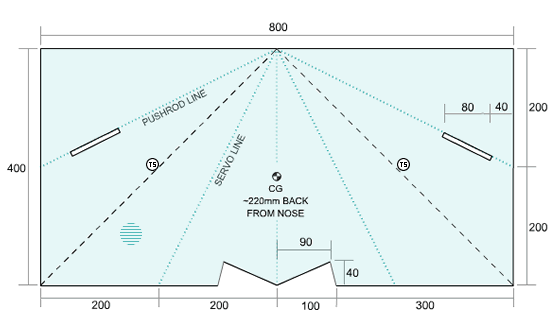
\includegraphics[height=5cm]{fotosNuevas/plan_main}
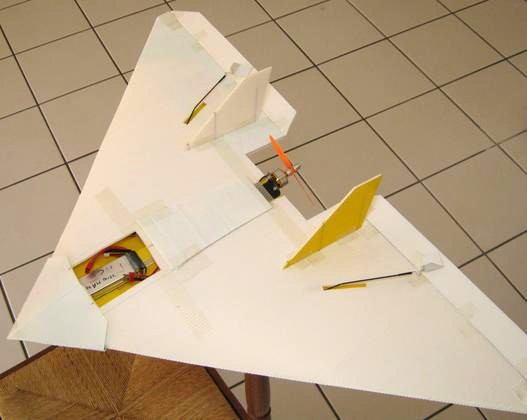
\includegraphics[height=5cm]{fotosNuevas/mugi02}}
\caption*{
Ejemplo del resultado que queremos obtener
}
\end{figure}

Además del diseño mecánico, nos interesa mucho explorar la parte de control software del avión. Normalmente, sería necesario adquirir una tarjeta controladora de vuelo para gestionar los motores que dan vida al robot.

Pero en este caso, nuestro proyecto va a optar por un enfoque completamente distinto. En concreto, vamos a basarnos en el trabajo que ha realizado George Walton en el \emph{Imperial College Robotics Society}. Su idea\footnote{\url{http://icrobotics.co.uk/wiki/index.php/UAV}} consiste en eliminar la tarjeta controladora y usar simplemente un smartphone viejo. Esto tiene sentido, ya que cualquier smartphone dispone de cámara, acelerómetros, brújula, GPS, etc. El proyecto de George nos proprociona una base estupenda para nuestro proyecto.

\subsubsection{Objetivos}

Aprender más sobre los aviones RC, la normativa vigente, el desarrollo de aplicaciones de navegación, etc. Además de fomentar el interés por los drones, el aeromodelismo autónomo y el reciclaje de circuitos y dispositivos móviles viejos. Dado su bajo coste, esperamos que más gente se una pronto al proyecto.

\subsubsection{Presupuesto}

Para este proyecto, debido a su naturaleza de bajo coste, no necesitaremos ni un control remoto, ni una tarjeta controladora: utilizaremos un teléfono móvil reciclado como cerebro del avión. Por tanto, solamente será necesario adquirir:

\begin{itemize}
\item \textbf{Lámina de plástico corrugado (160x40x0.4cm)} para construir la estructura, que cuesta 15\euro{}
\item \textbf{Baterías LiPo de 3 celdas}, que cuestan 21\euro{}/u. Compraremos 3 ya que se pueden reutilizas en muchos otros proyectos, es decir serán 63\euro{}
\item \textbf{Cargador de baterías LiPo} con los adaptadores adecuados, que cuesta 35\euro{}
\item \textbf{Motor brushless 3000kv} con driver y hélice propulsora, que cuesta 44\euro{}
\item \textbf{Gastos de envío del vendedor} para las baterías, el cargador, y el motor, serán 15\euro{}
\end{itemize}

Esto hace un total de {\bf 193\euro{}} para nuestro proyecto de avión RC autónomo de bajo coste




\subsection{Construcción de un Escáner 3D modelo Ciclop}

\subsubsection{Equipo de trabajo}
\begin{itemize}
\item Rodrigo Jiménez, estudiante de Telecomuniciones, EPS.
\item Pablo Moreno, estudiante de Informática-Matemáticas, EPS.
\item Víctor Uceda, estudiante de Informática-Matemáticas, EPS.
\end{itemize}
\subsubsection{Descripción}
 En el club de robótica se construyó en 2012 la primera impresora 3D open-source de la UAM. Queremos seguir siendo un referente tecnológico en este sentido, aprendiendo a construir herramientas modernas y automáticas que agilicen un tránsito veloz desde las ideas a los prototipos funcionales.

Creemos que la impresora 3D, junto a un escáner 3D y la fresadora Cyclone (que permite fresar circuitos electrónicos) son las herramientas modernas fundamentales para este proceso ágil.

\subsubsection{Objetivos}


\begin{wrapfigure}[11]{r}{6.5cm}\centering
    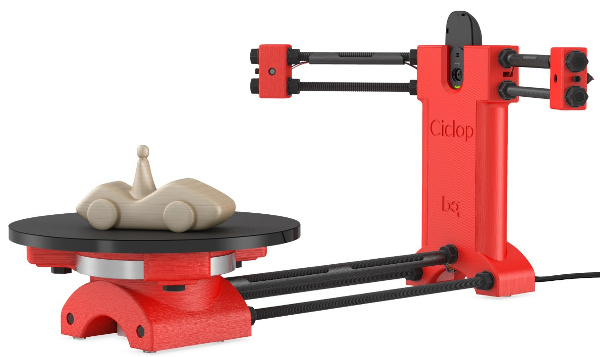
\includegraphics[scale=0.4]{fotos/bq-ciclop-1}
    \caption*{}
\end{wrapfigure}

Construcción del escáner 3D Ciclop diseñado y distribuido como kit de piezas por la empresa española BQ.\\
Además de adquirir una nueva herramiento de grandisima utilidad para el club, al ser un proyecto de construcción (ya que se compra el kit de piezas unicamente) tenemos el objetivo de aprender y profundizar en el diseño 3D, en la construcción de sistemas hardware y el software de escaneo y modelado 3D.
%\subsubsection{Contenido}

\subsubsection{Previsión de desarrollo}
La previsión de desarrollo del proyecto de montaje se estima en 2 semanas a partir del momento en el que el kit llegue al taller.\\
Con el escáner Ciclop ya montado comenzará la etapa de adaptación del software existente a los que equipos disponibles en el taller y la fase más importante de pruebas, calibrado y puesta a punto.
\subsubsection{Presupuesto}
La empresa BQ proporciona un kit completo de piezas los que nos permite acortar la étapa de adquisición de los materiales de forma muy notable e incluso ahorrar costes al adquirirlo todo a través de un mismo distribuidor.
El precio del kit es {\bf 249,90\euro{}} (con envío gratuito).
Enlace: \url{www.bq.com/es/ciclop}









\section{Organización de talleres formativos para alumnos de la Universidad}

\subsection{Taller: Introducción a las FPGAs libres con Verilog}
Las FPGAs son dispositivos empleados en aplicaciones que requieren velocidades de procesamiento muy elevadas debido a su alta potencia y reconfigurabilidad.
Recientemente se han desarrollado herramientas libres para trabajar con FPGAs, y desde el club de robótica queremos fomentar su uso ofreciendo uno de los primeros talleres del mundo en utilizarlas.

Queremos organizar el taller utilizando las placas \emph{iceStick} de Lattice Semiconductor:

\begin{figure}[hbtp]
\centerline{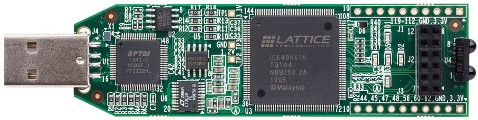
\includegraphics[width=0.75\linewidth]{fotos/icestick}}
\caption*{
Placa de desarrollo \emph{iceStick}
}
\end{figure}


Éstas placas tienen un coste muy reducido aún disponiendo de una FPGA de gran calidad. Además disponen de puerto USB para alimentación y datos, lo que las hace muy adecuadas para nuestro taller introductorio.

Para impartir el taller nos basaremos en los tutoriales que ha realizado Juan González\footnote{\url{https://github.com/Obijuan/open-fpga-verilog-tutorial/wiki}}, antiguo profesor de la EPS-UAM. Éstos proporcionan una introducción muy didáctica y fácil de entender.

\subsubsection{Contenido}

\begin{itemize}
	\item Introducción teórica a las FPGAs, con ejemplos de uso práctico y demostraciones
	\item Explicación de las diferencias entre los lenguajes VHDL y Verilog
	\item Propuesta de ejercicios introductorios para resolver en parejas (generadores de frecuencias audibles y con diodos LED, sistemas DAC con PWM, etc)
	\item Explicación de algunos ejemplos más avanzados (generación de señales de puerto serie, control de un conversor analógico-digital, etc).
	\item Propuesta del reto: control de un robot usando la FPGA. Los estudiantes aprenderán a integrar las entradas y las salidas usando descripciones de hardware en Verilog.
\end{itemize}

Impartir éstos contenidos complementaría muy bien las asignaturas de FPGAs que se ofrecen actualmente en los grados de Telecomuniciones e Informática, ya que los lenguajes de programación Verilog y VHDL son ampliamente empleados en la industria.


\subsubsection{Presupuesto}

Cada placa \emph{iceStick} cuesta 21.28\euro{}, y para el taller necesitaríamos 15 unidades. Por ello, el presupuesto estimado es \textbf{319.2\euro{}} (gastos de envío gratuitos).


\newpage



\chapter{Solicitud de subvención}


Como resumen de los proyectos propuestos y sus respectivos costes, a continuación proporcionamos una tabla:


\begin{tabular}{|l|l|l|}
\hline
 & \textit{\textbf{Concepto}}                          & \textit{\textbf{Presupuesto}} \\ \hline
1 & Presupuesto para mas cajas de proyecto				 & 80.25\euro{} \\ \hline
2 & Construcción de un avión RC autónomo               & 193\euro{} \\ \hline
3 & Taller: Introducción a las FPGAs libres con Verilog & 319.2\euro{} \\ \hline
4 & Construcción de un Escáner 3D modelo Ciclop        & 249.9\euro{} \\ \hline
 & \multicolumn{1}{|r|}{\textit{\textbf{Total:}}}      & \textit{\textbf{842.35\euro{}}}         \\ \hline
\end{tabular}


Desde la junta directiva del Club de Robótica nos comprometemos a promover todas las actividades aquí expuestas. Como entendemos que el presupuesto es limitado las hemos ordenado según su prioridad.






\end{document}
